	
\chapter*{\centering\large{1. Анализ факторов, влияющих на точность программно-имитационного моделирования}}
\addcontentsline{toc}{chapter}{1. Анализ факторов, влияющих на точность программно-имитационного моделирования}

 
\label{sec:Chapter1} \index{Chapter1}

\large{\begin{onehalfspace}

		
	\section*{\large{1.1 Классификация ошибок программно-имитационного моделирования}}
    \addcontentsline{toc}{section}{1.1 Классификация ошибок программно-имитационного моделирования}


   

	Процесс моделирования фокусируется на выделении реального изучаемого объекта, которым может являться, к примеру, какая-либо физическая система. Далее эта система заменяется моделью, то есть описанием, составленным с рядом допущений, определяющих погрешность итоговой оценки. Главной задачей модели является имитация характеристик и свойств оригинала, также поведение модели, которое зависит от параметров, которые определяют модель, должно отражать исследуемый процесс. Над моделью проводятся эксперименты и исследования, на основе которых делаются выводы о свойствах уже реального физического объекта.

   
	Основными требованиями, предъявляемыми к моделям, являются требования адекватности и применимости. Далее приведено уточнение их значения при построении моделей:
	\begin{enumerate}
	\item	Адекватность модели должна отражать важные для исследования, заданные свойства в физическом объекте с приемлемой точностью. Также необходимо выделить область адекватности модели, где погрешность расчёта меньше заданной предельно допустимой погрешности. Это подразумевает как оценку границ применимости физической модели, которая с рядом допущений описывает исследуемый процесс, так и оценку мощности вычислительной базы.
	
	\item	Применимость модели оценивает надёжность функционирования модели и полученных результатов расчёта. Важным условием описания модели является параметр времени. По отношению ко времени модели делят на динамические и статические. Статическое моделирование служит для описания состояния объекта в фиксированный момент времени, а динамическое для исследования объекта во времени.
 
	\end{enumerate} 

 Однако при применении программно-имитационного моделирования также появляются ошибки численного метода, связанные с неточностью численных схем, применяемых, например, при решении систем дифференциальных уравнений, а также ошибок реального времени, вызванных вычислительными ограничениями используемых технических средств.
Таким образом, сформирована следующая классификация ошибок \\ программно-имитационного моделирования:
\begin{enumerate}
	\item	ошибки физической модели;
\item	ошибки математической модели;
\item	ошибки численного метода;
\item	ошибки реального времени.
\end{enumerate} 

   
Схематично ошибки и порождающие их факторы представлены на рисунке 1. Далее они рассмотрены подробнее.
 
		\begin{center}
		\begin{figure}[h]
			\centering
			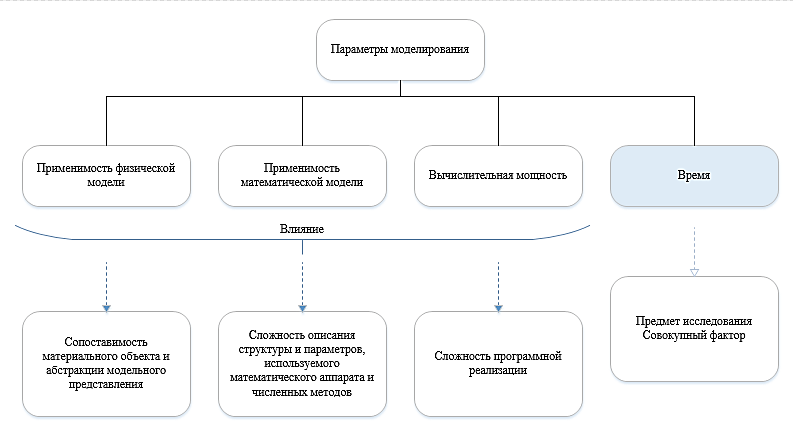
\includegraphics[width=0.9\linewidth]{mistake.png}
			\caption{Схема параметров, влияющих на расчёт модели}
			\label{fig:model2}
		\end{figure}
	\end{center}
     
    \section*{\large{1.2	Ошибки физической модели}}
    \addcontentsline{toc}{section}{1.2	Ошибки физической модели}
    Применение известной физической модели определяется заданием входных и выходных описывающих параметров и значений, которые связаны с исследуемыми характеристиками в различной степени значимости (некоторые факторы могут не закладываться в модель, в условиях определённой задачи, и не повлиять на качество целевых результатов моделирования). Однако неправильный выбор описания процесса с помощью физической модели может привести к критически упрощенной или усложнённой модели, а также дать весомую погрешность при оценке ключевых характеристик.



   
    
    \section*{\large{1.3 Ошибки математической модели }}
    \addcontentsline{toc}{section}{1.3 Ошибки математической модели }
    При переходе от физической модели к математической на результат влияет корректность постановки аналитической задачи и алгоритмы расчёта, используемые для получения конечного значения исследуемых характеристик, они вносят ошибку в значение. Этот этап имеет большое влияние на итоговую точность получаемого решения. Процесс перехода от физической модели можно контролировать сопоставлением моделируемых и экспериментальных данных. В частности, граничные условия математической модели строятся исходя из ограничений, накладываемых физической моделью, но при этом невозможно учесть фактор случайности величин, входящих в модель.
 


    \section*{\large{1.4	Ошибки численного метода}}
    \addcontentsline{toc}{section}{1.4	Ошибки численного метода}
   При программно-имитационном моделировании часто применяются численные методы, такие как методы Рунге-Кутты решения дифференциальных уравнений, итерационный метод и прочие. Ошибка данных методов хорошо изучена и для корректно поставленных задач может быть уменьшена до предела машинной точности, что точность моделирования практически всегда выше требуемого уровня. Однако увеличение точности при моделировании в реальном времени приводит к проявлению следующего вида ошибки.

    \section*{\large{1.5 Ошибки реального времени}}
    \addcontentsline{toc}{section}{1.5 Ошибки реального времени}
   Погрешность, вносимая вычислительной программой, зависит от выбора алгоритмов, применяемых при расчёте, а также от мощности платформы, на которой запущен процесс моделирования. 
Ошибка реального времени может быть определена как отклонение временной сетки программно-имитационной модели от временной сетки чистого численного моделирования.
Ошибка реального времени также может быть выражена в отклонении величины реального сигнала от сигнала, полученного путём чистого численного моделирования.




 
	


     
	\section*{\large{1.6 Особенности влияния ошибок при программно-имитационном моделировании}}
    \addcontentsline{toc}{section}{1.6	Особенности влияния ошибок при программно-имитационном моделировании}
	
	Одним из вариантов оценки процесса является построение имитационной модели, которая подразумевает логическое и алгоритмическое описание поведения отдельных блоков системы и правил их взаимодействия, согласно которым формируется процесс отображения событий в моделируемой системе \cite{sans26}.


 При моделировании поведения системы на вход модели даётся набор данных, который также можно понимать как набор состояний подсистем модели, далее в каждый момент времени исполнения модели происходит смена состояний подсистем, в зависимости от влияния внешних событий, которые модель обрабатывает, генерируя выходной поток данных.
 
 
 При таком способе моделирования необходимо следить за влиянием погрешности на корректность результатов модели. Далее представлены некоторые из вариантов, проявления описанного влияния:
 
	\begin{enumerate} 
 
		\item погрешность моделирования шкалы времени влияет на результаты моделирования, это может быть важно при описании синхронных процессов;
		\item проявляется отклонение модельного времени от реального, это может быть важно при описании взаимодействия систем, состояние которых изменяется разово в каждый момент времени, само же модельное время сдвигается на заданную величину отсчёта и в результате точность моделирования времени соблюдается с точностью до величины сдвига;
		\item результаты моделирования зависят от выбранного способа расчёта модели.

	\end{enumerate} 


 
	
	
	
	\section*{\large{1.7 Рассмотрение факторов, влияющих на точность программно-имитационного моделирования на примере моделирования маятника}}
   \addcontentsline{toc}{section}{1.7 Рассмотрение факторов, влияющих на точность программно-имитационного моделирования на примере моделирования маятника}
	
	
	Малые колебания физического тела можно свести к математическому маятнику с помощью приближения гармоническим осциллятором с малой амплитудой и возвращающей силой, пропорциональной отклонению от положения равновесия. 
 
    Моделирование процесса колебания маятника является классической задачей инженерии. При моделировании маятника несколько факторов могут внести погрешность в итоговые значения времени затухания, изменения периода колебаний (из-за внешнего воздействия на систему) и других параметров. Ниже приведены некоторых из таких параметров:

    \begin{enumerate} 
    
    \item  Длина нити маятника является одним из основных параметров, влияющих на период колебаний. Масса и распределение массы вокруг точки подвеса также могут внести погрешность.

    \item Наличие воздушного трения может вызвать затухание колебаний маятника. Маятник может испытывать нелинейности, такие как упругость нити, нелинейное трение или нелинейные связи между массой и подвесом.

    \item Маятник может подвергаться воздействию внешних сил, таких как ветер или другие механические воздействия. В реальных маятниках часть энергии может диссипироваться в виде тепла из-за трения, сопротивления воздуха и других факторов. Это может привести к затуханию колебаний и изменению периода колебаний с течением времени.

   \item Начальные условия, такие как амплитуда и начальная скорость, также могут внести погрешность в моделирование. 

    \end{enumerate}
    
    Таким образом, помимо факторов, определяющих моделируемый процесс колебаний реального физического тела с заданными геометрическими параметрами, а также модулем упругости, вклад в итоговую модель вносят параметры самой модели эквивалентного маятника.

    
    Рассмотрим модель колебательного процесса на примере физического маятника — осциллятора, представляющего собой твёрдое тело, совершающее колебания в поле каких-либо сил относительно точки, не являющейся центром масс этого тела, или неподвижной оси, перпендикулярной направлению действия сил и не проходящей через центр масс этого тела. 
    
    Однако и такую систему можно упростить переходом к модели математического маятника, которая и служит простейшей моделью физического тела, совершающего колебания, но эта модель не учитывает распределение массы в объёме тела \cite{maytnik29}. Для связи между малыми колебаниями физического тела и моделируемым математическим маятником необходимо рассчитать эквивалентное значение момента инерции, в который закладывается учет массы и геометрии тела.


    Для перехода к математическому маятнику, необходимо учесть следующие факторы:

\begin{enumerate} 
\item  приведённая длина подвесной нити  математического маятника выбирается так, чтобы период колебаний совпадал с периодом малых колебаний физического тела, что является определяющим параметром модели;


\item  в реальных системах существуют внешние силы, такие как трение и сопротивление воздуха. Они могут быть учтены в модели математического маятника путем введения демпфирования или добавления дополнительных сил сопротивления.

\end{enumerate}


Следуя этим принципам, физическое тело с малыми колебаниями можно представить в виде математическим маятником, что позволяет использовать известные формулы и методы решения для анализа и предсказания поведения системы. Алгоритм перехода к имитационной модели кратко показан на рисунке 2.

 
 
	\begin{center}
		\begin{figure}[h]
			\centering
				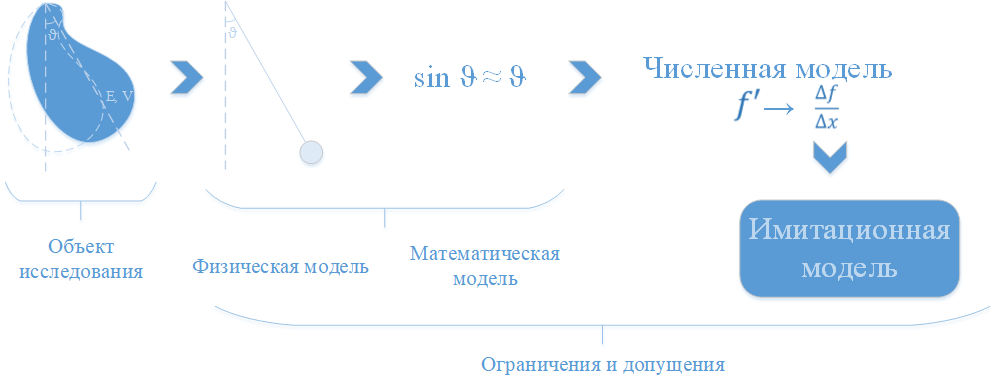
\includegraphics[width=1\linewidth]{pendim.png}
			\caption{Пример моделирования колебаний}
			\label{fig:model3}
		\end{figure}
	\end{center}
 

   
 
 Таким образом, модель сводится к системе, состоящей из материальной точки, висящей на нерастяжимой невесомой нити в однородном поле тяжести, но подвес неидеален в нём присутствует постоянное трение, которое вызывает затухания, процесс затухания колебания можно исследовать с помощью программно-имитационного моделирования. Для демонстрации погрешности моделирования используется численная модель, разработанная в среде Matlab+Simulink. Схема модели представлена на рисунке 3. Модельное (компьютерное) время должно соответствовать теоретическому времени, с точностью до заданных на каждом этапе разработки допущений и погрешностей. Модель используется в качестве примера перехода от структурной схемы к расчетной с помощью вычислительного моделирования. 


Согласно схеме, приведённой на рисунке 1, факторами влияющими на моделирование колебательного движения заданного физического объекта являются:
	
	\begin{enumerate} 	
	\item Соответствие применяемой теории колебаний математического маятника к малым колебания физического тела. Появляется временная составляющая, зависящая от законов задающих параметры колебаний (к примеру, зависимость периода колебаний модельного маятника от его приведённой длины).
		
	\item Сложность поиска аналитического решения при наличии затухания в системе, величина которого изменяет по неизвестному закону (расчёт параметров вычислительной модели представляет результат решения систему дифференциальных уравнений в момент времени, соответственно в зависимости от схемы решения и возможности решить систему аналитически зависит время модели).
	
	\item  Оценка возможности замедления (или ускорения)
	временной шкалы, при постановке, к примеру, длительного по времени эксперимента (специфика процесса, может быть неоднородна по времени, возможность динамически менять параметры системы, также влияет на результат). 
	\end{enumerate} 

 \begin{center}
		\begin{figure}[h]
			\centering
			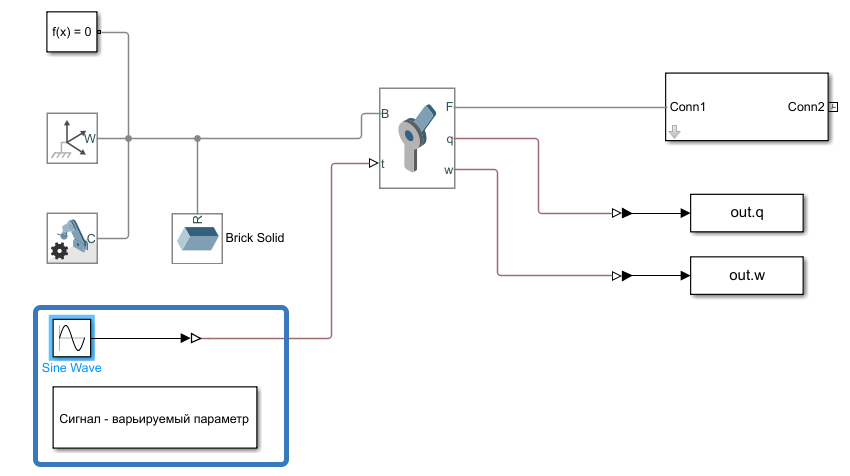
\includegraphics[width=0.85\linewidth]{pend3.png}
			\caption{Модель маятника в Simulink}
			\label{fig:model4}
		\end{figure}
	\end{center}

	

		
	В рассматриваемом примере при выбранном способе расчёта моделирования (перехода к разностной схеме для расчёта), контролируемыми параметрами модели является ее визуальное отображение и значение вектора в пространстве состояний. Таким образом, определяющим погрешность времени фактором является неточность описания состояния в фазовом пространстве состояний, а также неточность расчета физической модели, возникающая из выбранного решателя и его согласования с визуализацией.

	Полученная модель должна давать результат сопоставимый с реальностью при наложенных на нее ограничениях, для проверки этого производится её численный обсчет на разных параметрах. 
	
	

 
\end{onehalfspace}}
